\documentclass{beamer}
\usepackage[ngerman]{babel}
\usepackage[utf8]{inputenc}
\usetheme{Boadilla}

\usepackage{savesym}
\savesymbol{checkmark}
\usepackage{dingbat}
\usepackage{dirtytalk}
\usepackage{tikz}
\usetikzlibrary{positioning}
\usepackage{changepage}

\begin{document}
\title{Digitalisierung}
\subtitle{Grundlagenfach Informatik}
%\subtitle{Freifach Informatik}
%\subtitle{Berufsfeldfach Informatik}
%\subtitle{Ergänzungsfach Informatik}
\author{Oliver Probst (pro@kwse.ch)}
\institute{KSWE}
\date{11. August 2022}
\titlegraphic{
\includegraphics[scale=0.5]{graphics/kswe_logo.pdf}}

\begin{frame}
\titlepage
\end{frame}

\frame[c]{\frametitle{Willkommen}
\begin{center}
\Huge Ginf F1C
\end{center}
}

\frame{\frametitle{Was ist Informatik?}
\begin{definition}[Informatik]
Die Informatik ist die Wissenschaft der systematischen, automatisierten Verarbeitung von \textbf{Information}, der \textbf{Informationsspeicherung}, Informationsverwaltung und \textbf{Informationsübertragung}.
\end{definition}
}

\frame{\frametitle{Was machen Informatiker?}
\begin{figure}
\includegraphics[scale=0.5]{graphics/bs4}
\caption{BatScope\footnote{\url{http://batscope.ch}}}
\end{figure}
}

\frame{\frametitle{Was machen Informatiker?}
\begin{figure}
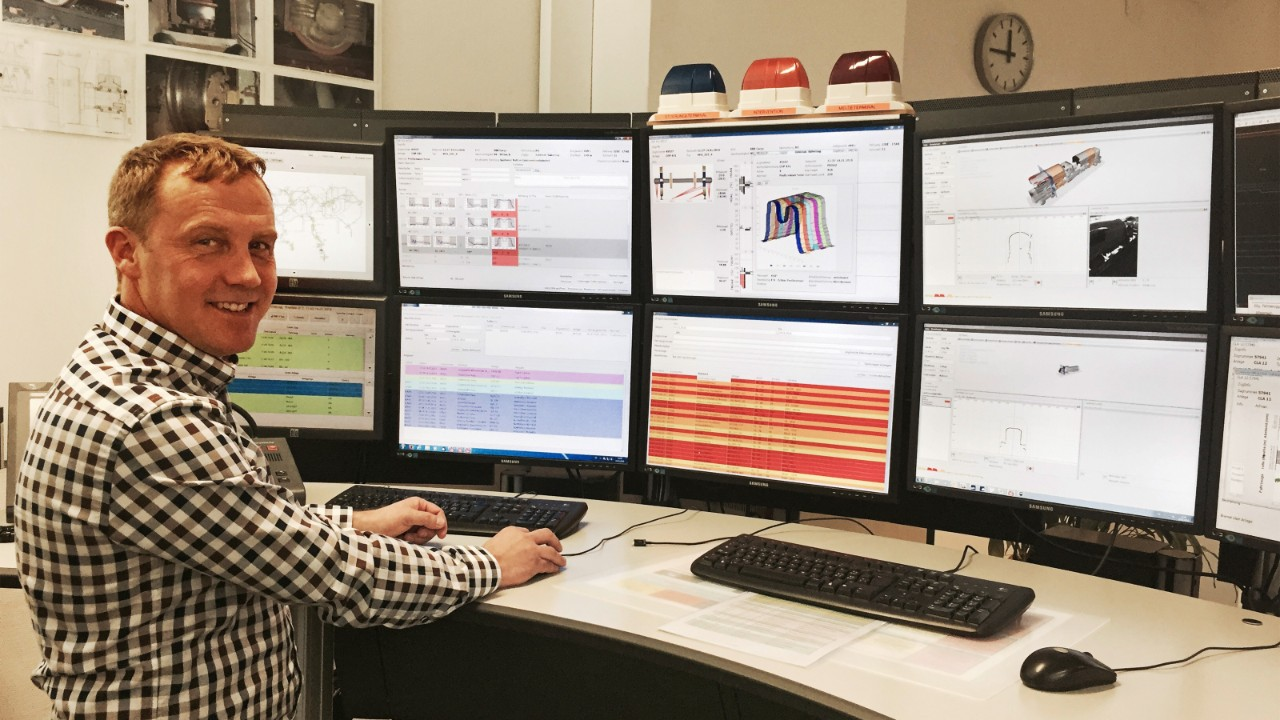
\includegraphics[scale=0.25]{graphics/zke}
\caption{Zugkontrolleinrichtungen (ZKE)\footnote{Präsentation der Anlagen via Microsoft Teams}}
\end{figure}
}

\frame{\frametitle{Wie wird man Informatiker?}
\begin{itemize}
\item
\item
\item
\end{itemize}
}


\frame{\frametitle{Warum Informatik?}
\begin{itemize}
\item Die von Menschen erzeugte Welt verstehen und mitgestalten lernen.
\item Denkweisen des Engineering verstehen und anwenden.
\item Grundkompetenzen in Mathematik und Sprachen stärken.
\end{itemize}
}

\frame{\frametitle{Warum Informatik?}
\begin{figure}

\includegraphics{graphics/eth}
\caption{Vorbereitung auf das Studium}
\end{figure}
}

\frame{\frametitle{Bachelor-Studiengänge an der ETH}
\begin{itemize}
\item Architektur
\item Bauingenieurwissenschaften, Umweltingenieurwissenschaften, Raumbezogene Ingenieurwissenschaften
\item Biologie, Pharmazeutische Wissenschaften, Gesundheitswissenschaften und Technologie
\item Chemie, Chemieingenieurwissenschaften, Interdisziplinäre Naturwissenschaften
\item Erd- und Klimawissenschaften \rightpointleft
\item Staatswissenschaften (Berufsoffiziere) \rightpointleft
\item Humanmedizin
\item Agrarwissenschaften, Lebensmittelwissenschaften, Umweltnaturwissenschaften
\item Informatik
\item Elektrotechnik und Informationstechnologie
\item Maschineningenieurwissenschaften
\item Materialwissenschaft
\item Mathematik, Physik
\end{itemize}
}

\frame[t]{\frametitle{Organisation bis zur Vario-Woche}
\textbf{Roadmap}: Wir erarbeiten zunächst ein paar Grundlagen (Theorie) bevor wir nach den Herbstferien mit dem Programmieren (Praxis) beginnen.
\begin{itemize}
\item 6 Unterrichtslektionen à 90 Minuten
\begin{itemize}
\item Sie erhalten alle Unterrichtsunterlagen (Skripte, Übungen, Lösungen etc.) schriftlich (ausgedruckt und/oder digital).
\item Vieles ist bereits von mir dokumentiert. Machen Sie sich ggf. Notizen direkt in den Unterlagen.
\item Übungen handschriftlich direkt in den Unterlagen lösen.
\end{itemize}
\item 1 Prüfungslektion (22. September 2022) à 90 Minuten
\begin{itemize}
\item Schriftliche Prüfung \textbf{ohne} Computer.
\item Hilfsmittel: Taschenrechner
\item Sie erhalten die Lernziele schriftlich.
\end{itemize}
\end{itemize}
\begin{center}
\huge Fragen?
\end{center}
}

\frame[t]{\frametitle{Hinweise, Tipps und Regeln}
\begin{itemize}
\item Machen Sie auf sich aufmerksam, falls Sie etwas nicht verstehen.
\item Fragen Sie nach, falls ich etwas vergesse.
\item Melden Sie sich, falls ich (noch) eine Aufgabe vorlösen soll.
\item Lösen Sie die Aufgaben möglichst selbstständig.
\item Lesen Sie die Unterlagen möglichst zeitnah zur Wiederholung (nicht erst vor der Prüfung).
\item Der Computer ist (zumindest im Informatikunterricht) ein Arbeitsgerät.
\item Bitte folgen Sie aufmerksam, wenn ich etwas am Computer vorzeige.
\item Wir machen $10$ Minuten Pause.
\item Wir achten auf eine angenehme Arbeitsatmosphäre im Klassenzimmer (Lautstärke, Trinken, Essen etc.).
\item Schauen Sie am Abend \textbf{vor} dem Unterricht ins Microsoft Teams. Ich schreibe Ihnen dort eine Nachricht, falls wir das Notebook \textbf{nicht} brauchen.
\end{itemize}
}

\frame{\frametitle{Worum geht es?}\framesubtitle{Informationsspeicherung}
\begin{adjustwidth}{-1ex}{-1ex}
\begin{figure}[htb]
\centering
\begin{tikzpicture}
\node[inner sep=0pt] (portland) at (-4.5,0) {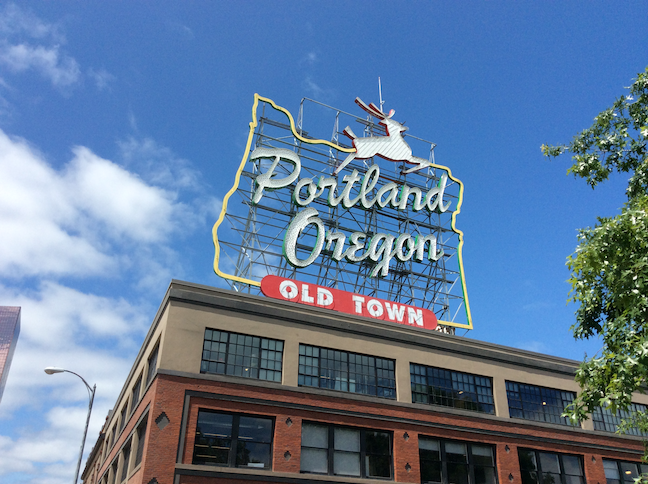
\includegraphics[height=2.5cm]{graphics/portland}};
\node[inner sep=0pt] (applekameraicon) at (0,0) {
\includegraphics[scale=0.1]{graphics/apple-kamera-icon}};
\node[inner sep=0pt] (smartphonefestplatte) at (4.5,0) {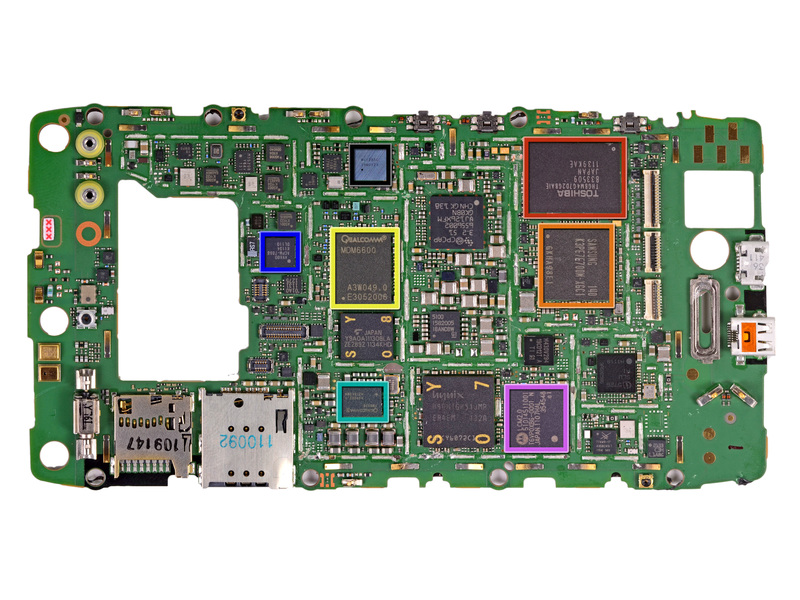
\includegraphics[height=2.5cm]{graphics/smartphone_festplatte}};
\draw[-latex, thick] (portland) -- (applekameraicon) node[midway, fill=white] {\say{Klick}};
\draw[-latex, thick] (applekameraicon) -- (smartphonefestplatte) node[midway, fill=white] {
\includegraphics[scale=0.15]{graphics/image_file_icon}};
\end{tikzpicture}
\end{figure}
\end{adjustwidth}
}

\frame[t]{\frametitle{Informationsspeicherung}\framesubtitle{Was ist eine Datei?}
\begin{definition}[Datei]
In einer Datei (engl. file) kann ein Computer Daten langfristig auf einem Speichermedium (Festplatte, USB-Stick, Smartphone-Speicher etc.) unter einem Namen speichern. Die gespeicherten Informationen in der Datei können sehr vielseitig sein: Texte, Bilder, Audio, Video, \dots . Dateien bleiben nach einem Neustart des Computers erhalten und werden nicht gelöscht.
\end{definition}

\vspace{1cm}

\begin{definition}[Bilddatei]
Eine Datei, in der ein Bild gespeichert ist, nennen wir Bilddatei.
\end{definition}
}

\frame[t]{\frametitle{Informationsspeicherung}\framesubtitle{Was ist eine Dateinamen-Erweiterung?}
\begin{definition}[Dateinamen-Erweiterung]
Ein Dateiname wird unter Verwendung eines Punktes (\texttt{.}) in zwei Teile gegliedert, den eigentlichen Namen und die sogenannte Dateinamen-Erweiterung (engl. file extension).
\end{definition}
}

\frame{\frametitle{Worum geht es?}\framesubtitle{Reduktion der Datengrösse}
\begin{figure}[htb]
\centering
\begin{minipage}{0.45\textwidth}
\centering
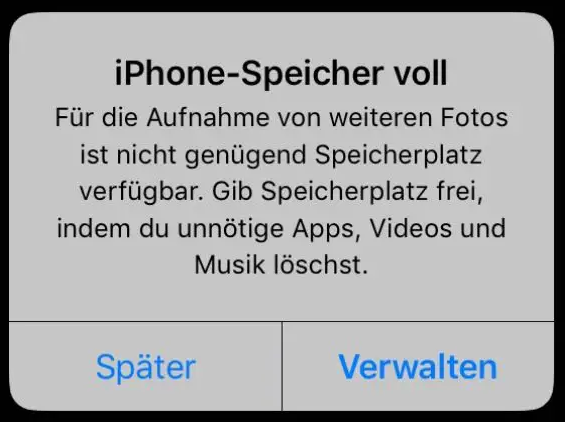
\includegraphics[height=3.5cm]{graphics/iphone_speicher_voll}
\end{minipage}
\hfill
\begin{minipage}{0.45\textwidth}
\centering
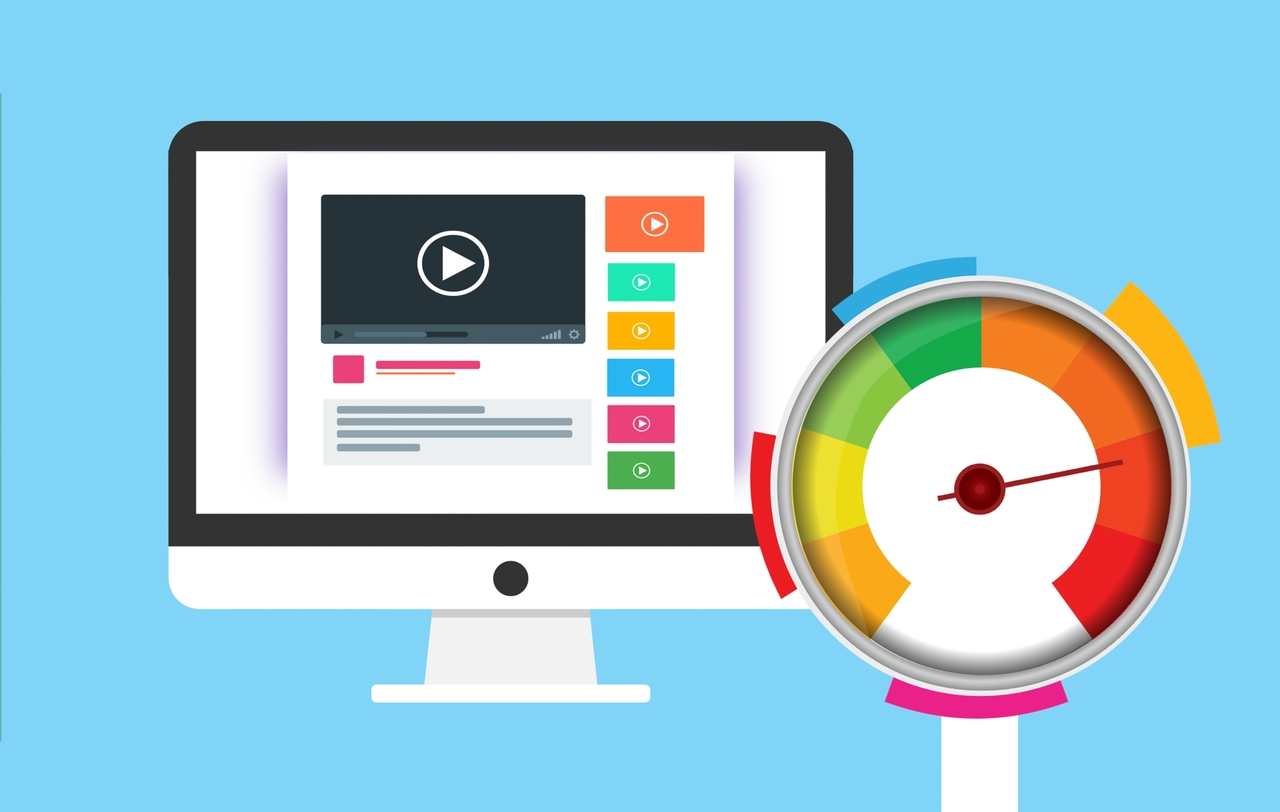
\includegraphics[height=3.5cm]{graphics/internet_speed}
\end{minipage}
\end{figure}
}

\frame{\frametitle{Worum geht es?}\framesubtitle{Fehlererkennung und Fehlerkorrektur bei der Datenübertragung}
\begin{figure}[htb]
\centering
\begin{tikzpicture}
\node[inner sep=0pt] (sender) at (-4,0) {
\includegraphics[height=2cm]{graphics/lego_alice}};
\node[inner sep=0pt] (empfaenger) at (4,0) {
\includegraphics[height=2cm]{graphics/lego_bob}};
\node[below=0.5cm of sender] {Sender (Alice)};
\node[below=0.5cm of empfaenger] {Empfänger (Bob)};
\node[inner sep=0pt, red] (fehler) at (0,-1) {Fehler};
\draw[-latex, thick] (sender) -- (empfaenger) node[midway, fill=white] {\say{Datenübertragung}};
\draw[-latex, thick, red] (fehler) -- (0,-0.1);
\end{tikzpicture}
\end{figure}
}

\end{document}